%\documentclass{article}
%\usepackage{graphicx,subfigure}
%\begin{document}

\begin{figure}[h]
  \centering
   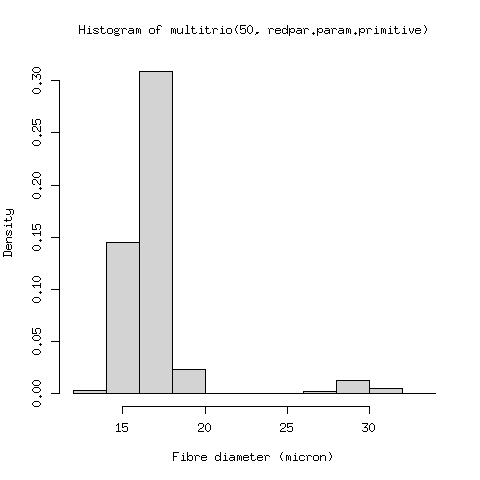
\includegraphics[width=0.9\textwidth]{diamhistprimitive.png}
  \caption{Histogram of fibre diameter for 50 trio groups modelled with the {\em trio()} software with the same parameters as Table~\ref{tab:triolp} except papilla cells per follicle altered to Pc=160, Pl=150, So=40, Sd=35 to simulate a primitive 2-coated fleece}
  \label{fig:diamhistprimitive}
\end{figure}

%\end{document}

